\documentclass[12pt]{report}
\usepackage[utf8]{inputenc}
\usepackage[russian]{babel}
%\usepackage[14pt]{extsizes}
\usepackage{listings}
\usepackage{graphicx}
\usepackage{amsmath,amsfonts,amssymb,amsthm,mathtools} 
\usepackage{pgfplots}
\usepackage{filecontents}
\usepackage{float}
\usepackage{comment}
\usepackage{indentfirst}
\usepackage{eucal}
\usepackage{pdfpages}
\usepackage{enumitem}
%s\documentclass[openany]{book}
\frenchspacing

\usepackage{indentfirst} % Красная строка

\usetikzlibrary{datavisualization}
\usetikzlibrary{datavisualization.formats.functions}

\usepackage{amsmath}


% Для листинга кода:
\lstset{ %
	language=c,                 % выбор языка для подсветки (здесь это С)
	basicstyle=\small\sffamily, % размер и начертание шрифта для подсветки кода
	numbers=left,               % где поставить нумерацию строк (слева\справа)
	numberstyle=\tiny,           % размер шрифта для номеров строк
	stepnumber=1,                   % размер шага между двумя номерами строк
	numbersep=5pt,                % как далеко отстоят номера строк от подсвечиваемого кода
	showspaces=false,            % показывать или нет пробелы специальными отступами
	showstringspaces=false,      % показывать или нет пробелы в строках
	showtabs=false,             % показывать или нет табуляцию в строках
	frame=single,              % рисовать рамку вокруг кода
	tabsize=2,                 % размер табуляции по умолчанию равен 2 пробелам
	captionpos=t,              % позиция заголовка вверху [t] или внизу [b] 
	breaklines=true,           % автоматически переносить строки (да\нет)
	breakatwhitespace=false, % переносить строки только если есть пробел
	escapeinside={\#*}{*)}   % если нужно добавить комментарии в коде
}


\usepackage[left=2cm,right=2cm, top=2cm,bottom=2cm,bindingoffset=0cm]{geometry}
% Для измененных титулов глав:
\usepackage{titlesec, blindtext, color} % подключаем нужные пакеты
\definecolor{gray75}{gray}{0.75} % определяем цвет
\newcommand{\hsp}{\hspace{20pt}} % длина линии в 20pt
% titleformat определяет стиль
\titleformat{\chapter}[hang]{\Huge\bfseries}{\thechapter\hsp\textcolor{gray75}{|}\hsp}{0pt}{\Huge\bfseries}


% plot
\usepackage{pgfplots}
\usepackage{filecontents}
\usetikzlibrary{datavisualization}
\usetikzlibrary{datavisualization.formats.functions}

\begin{document}
	%\def\chaptername{} % убирает "Глава"
	\thispagestyle{empty}
	\begin{titlepage}
		\noindent \begin{minipage}{0.15\textwidth}
			
\includegraphics[width=\linewidth]{b_logo}
		\end{minipage}
		\noindent\begin{minipage}{0.9\textwidth}\centering
			\textbf{Министерство науки и высшего образования Российской Федерации}\\
			\textbf{Федеральное государственное бюджетное образовательное учреждение высшего образования}\\
			\textbf{~~~«Московский государственный технический университет имени Н.Э.~Баумана}\\
			\textbf{(национальный исследовательский университет)»}\\
			\textbf{(МГТУ им. Н.Э.~Баумана)}
		\end{minipage}
		
		\noindent\rule{18cm}{3pt}
		\newline\newline
		\noindent ФАКУЛЬТЕТ $\underline{\text{«Информатика и системы управления»}}$ \newline\newline
		\noindent КАФЕДРА $\underline{\text{«Программное обеспечение ЭВМ и информационные технологии»}}$\newline\newline\newline\newline\newline
		
		\begin{center}
			\noindent\begin{minipage}{1.1\textwidth}\centering
				\Large\textbf{Отчет по лабораторной работе №8}\newline
				\textbf{по дисциплине <<Функциональное и логическое}\newline
				\textbf{~~~программирование>>}\newline\newline
			\end{minipage}
		\end{center}
		
		\noindent\textbf{Тема} $\underline{\text{Структура программы на Prolog и ее реализация~~~~~~~~~~~~~~~~~~~~~}}$\newline\newline
		\noindent\textbf{Студент} $\underline{\text{Золотухин А.В.~~~~~~~~~~~~~~~~~~~~~~~~~~~~~~~~~~~~~~~~~~~~~~~~~~~~~~~~~~~~~~~~~}}$\newline\newline
		\noindent\textbf{Группа} $\underline{\text{ИУ7-64Б~~~~~~~~~~~~~~~~~~~~~~~~~~~~~~~~~~~~~~~~~~~~~~~~~~~~~~~~~~~~~~~~~~~~~~~~~}}$\newline\newline
		\noindent\textbf{Оценка (баллы)} $\underline{\text{~~~~~~~~~~~~~~~~~~~~~~~~~~~~~~~~~~~~~~~~~~~~~~~~~~~~~~~~~~~~~~~~~~~~~~~~}}$\newline\newline
		\noindent\textbf{Преподаватель} $\underline{\text{Толпинская Н.Б., Строганов Ю. В.~~~~~~~~~~~~~~~~~~~~~~~~~~}}$\newline\newline\newline
		
		\begin{center}
			\vfill
			Москва~---~\the\year
			~г.
		\end{center}
	\end{titlepage}
	
	
	\section*{Задание 1}
	Создать базу знаний «Собственники», дополнив (и минимально изменив) базу
	знаний, хранящую знания:
	\begin{itemize}
	\item <<Телефонный справочник>>: Фамилия, №тел, Адрес – структура (Город, 
	Улица, №дома, №кв),
	\item <<Автомобили>>: Фамилия владельца, Марка, Цвет, Стоимость, и др.,
	\item <<Вкладчики банков>>: Фамилия, Банк, счет, сумма, др.,
	\end{itemize}
	знаниями о дополнительной собственности владельца. Преобразовать знания об 
	автомобиле к форме знаний о собственности.
	Вид собственности (кроме автомобиля):
	\begin{itemize}
	\item Строение, стоимость и другие его характеристики;
	\item Участок, стоимость и другие его характеристики;
	\item Водный транспорт, стоимость и другие его характеристики.
	\end{itemize}

	Описать и использовать вариантный домен: Собственность. Владелец может иметь, но 
	только один объект каждого вида собственности (это касается и автомобиля), или не 
	иметь некоторых видов собственности. 
	
	Используя конъюнктивное правило и разные формы задания одного вопроса (пояснять 
	для какого задания – какой вопрос), 
	обеспечить возможность поиска:
	\begin{enumerate}
		\item Названий всех объектов собственности заданного субъекта,
		\item Названий и стоимости всех объектов собственности заданного субъекта,
		\item Разработать правило, позволяющее найти суммарную стоимость всех 
		объектов собственности заданного субъекта.
	\end{enumerate}

	Для 2-го пункт и одной фамилии составить таблицу, отражающую конкретный 
	порядок работы системы, с объяснениями порядка работы и особенностей использования 
	доменов (указать конкретные Т1 и Т2 и полную подстановку на каждом шаге)
	
	
	\subsection*{Решение}
	\begin{lstlisting}
domains

city, street = string.
house, flat = integer.
struct_address = address(city, street, house, flat).
surname = string.
phone = integer.
model, color = string.
price, year = integer.
bank = string.
sum, account = integer.
size = integer.

ownership = building(price, struct_address);
area(price, size);
water_transport(price, color);
car(price, model, color).

predicates

phone_record(surname, phone, address_struct).
depositor(surname, bank, account, sum).
own(surname, ownnership).
findOwnershipsNamePriceBySurname(surname, string, price).
sumOwnershipsPriceHelp(surname, string, price).
sumOwnershipsPrice(surname, price).

clauses

phone_record(rich, 7777772, address(london, green, 1, 10)).
phone_record(rich, 7777771, address(london, green, 1, 10)).
phone_record(rich, 1111111, address(moscow, zelenaya, 2, 20)).
phone_record(middle, 9999999, address(moscow, ivanovskaya, 3, 2)).
phone_record(poor, 3333331, address(karaganda, pit, 23, 5)).
phone_record(poor, 3333332, address(perm, pit, 36, 7)).
phone_record(poor, 3333333, address(kop,leet, 2, 53)).

car(rich, coolmodel, red, 1000000, 123456).
car(rich, coolestmodel, green, 5000000, 837495).
car(rich, coolestmodel, blue, 5000000, 836472).
car(middle, awesommodel, red, 1000000, 047163).

depositor(rich, gosbank, 10, 10000000).
depositor(rich, mosbank, 15, 9000000).
depositor(middle, mosbank, 17, 20000).
depositor(middle, newbank, 345, 0).

own(rich, building(100, address(kop, leet, 2, 53))).
own(rich, area(10, 500)).
own(rich, water_transport(1, green)).
own(rich, car(5, model1, red)).

own(middle, car(3, model2, red)).
own(middle, building(90, address(moscow, leninskaya, 2, 53))).

findOwnershipsNamePriceBySurname(S, building, P) :- own(S, building(P, _)).
findOwnershipsNamePriceBySurname(S, area, P) :- own(S, area(P, _)).
findOwnershipsNamePriceBySurname(S, water_transport, P) :- own(S, water_transport(P, _)).
findOwnershipsNamePriceBySurname(S, car, P) :- own(S, car(P, _, _)).

sumOwnershipsPriceHelp(S, building, P) :- own(S, building(P, _)).
sumOwnershipsPriceHelp(S, area, P) :- own(S, area(P, _)).
sumOwnershipsPriceHelp(S, water_transport, P) :- own(S, water_transport(P, _)).
sumOwnershipsPriceHelp(S, car, P) :- own(S, car(P, _, _)).

sumCost(S, P) :- sumCostInner(S, building, P1), sumCostInner(S, area, P2), sumCostInner(S, water_transport, P3), sumCostInner(S, car, P4), P = P1 + P2 + P3 + P4.

goal

findOwnershipsNamePriceBySurname(middle, Ownnership, Price).


	\end{lstlisting}

	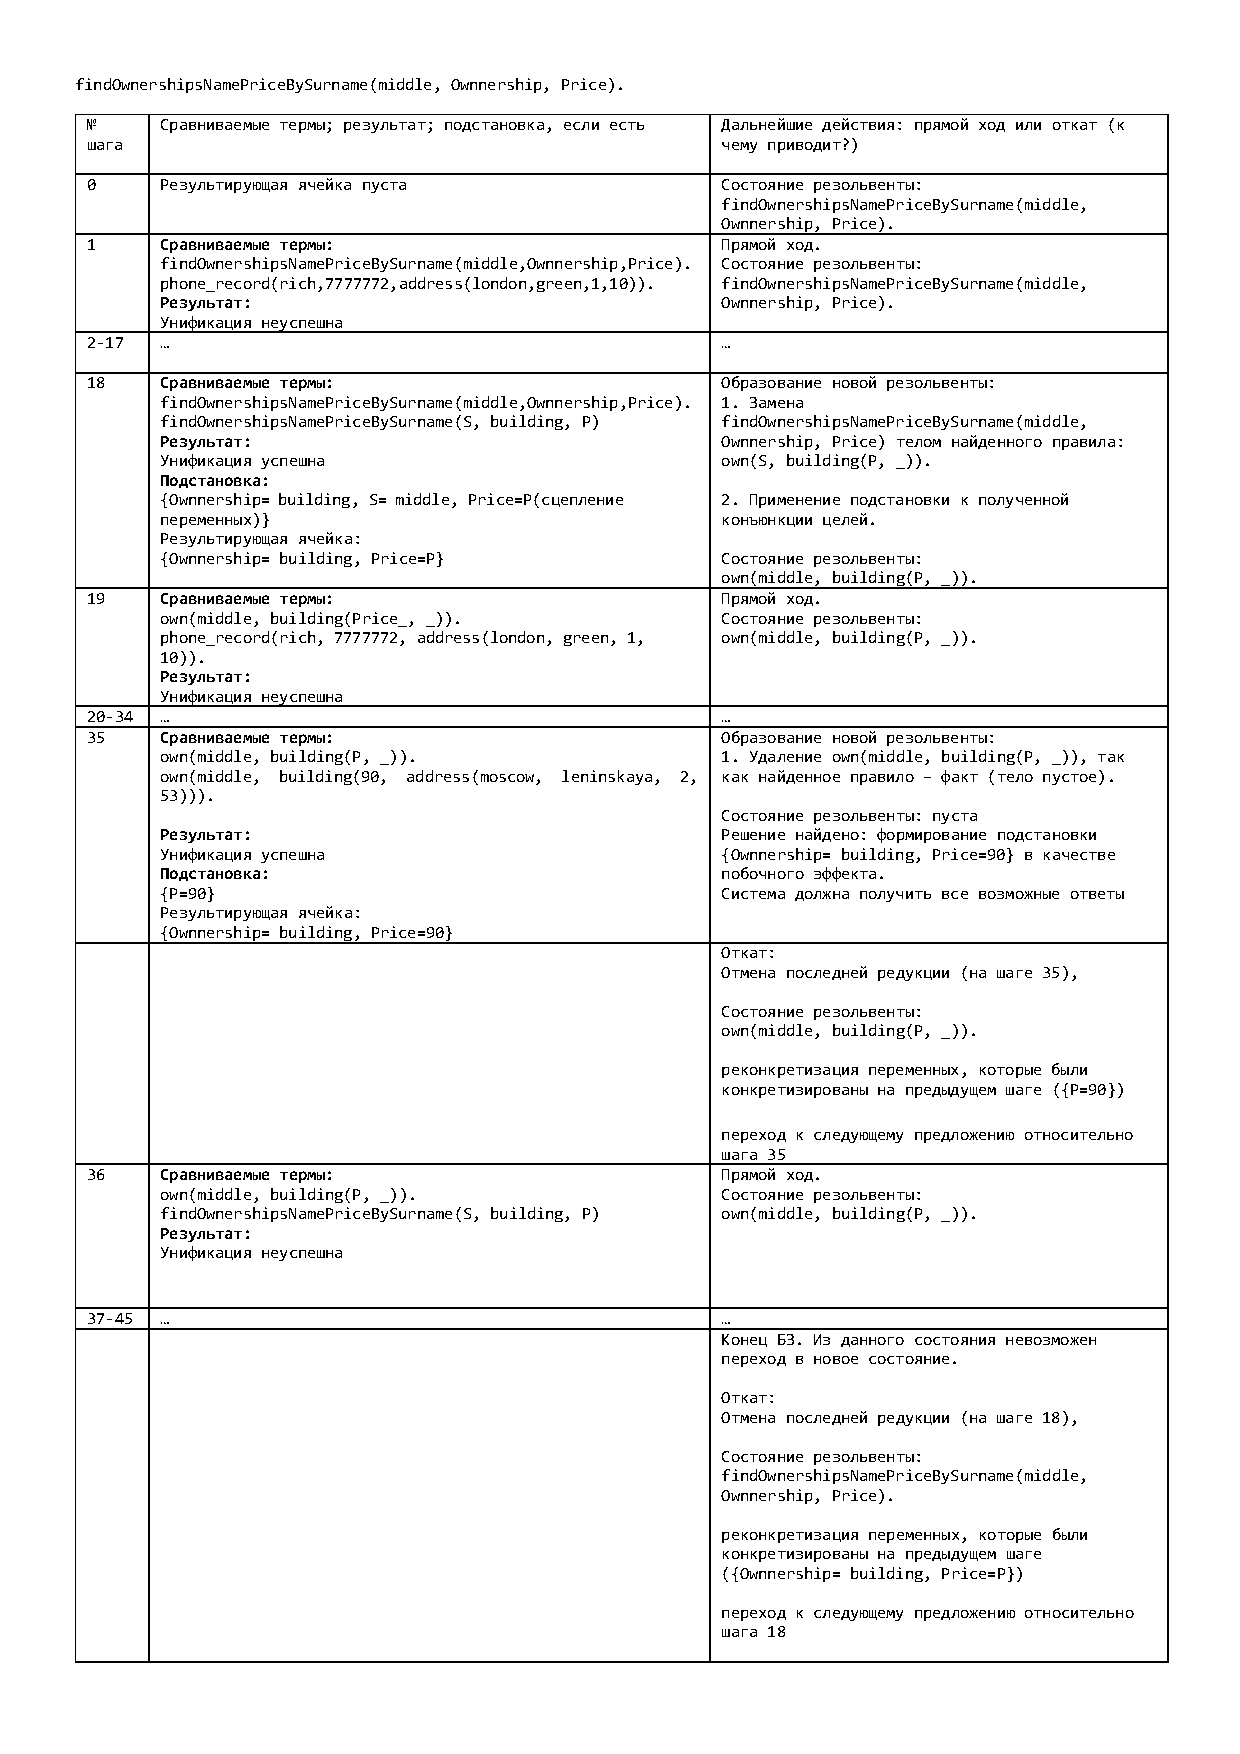
\includepdf[pages=-]{report_extra.pdf}

	\bibliographystyle{utf8gost705u}  % стилевой файл для оформления по ГОСТу
	\bibliography{51-biblio}          % имя библиографической базы (bib-файла)
	
\end{document}